\documentclass[aspectratio=43]{beamer}

\usepackage[utf8]{inputenc}
\usepackage[T1]{fontenc}
\usepackage[brazil]{babel}
\usepackage{graphicx}
\usepackage{array}
\usepackage{tikz}
\usetikzlibrary{arrows.meta, positioning, shapes.geometric}
\usepackage{booktabs}
\usepackage{amsmath}

\setbeamertemplate{itemize item}{$\bullet$}
\setbeamertemplate{itemize subitem}{$\circ$}

% Coluna alinhada à esquerda sem hifenização excessiva
\newcolumntype{P}[1]{>{\raggedright\arraybackslash}p{#1}}

% Paleta institucional UEL
\definecolor{uelgreen}{RGB}{15, 80, 35}
\definecolor{uelaccent}{RGB}{34, 115, 58}

\setbeamercolor{boxcinza}{bg=gray!10}
\setbeamercolor{boxtitulo}{bg=gray!25}
\setbeamercolor{boxcorpo}{bg=gray!10}

\setbeamertemplate{navigation symbols}{}
\setbeamertemplate{headline}{
  \begin{beamercolorbox}[wd=\paperwidth,ht=0.30cm,dp=0.15cm]{headline}
    \color{white}
    \hspace{0.3cm}Mineração de Dados (2COP024) -- Previsão de Avaliações Negativas
    \hfill \insertframenumber\ de \inserttotalframenumber \hspace{0.3cm}
  \end{beamercolorbox}
}
\setbeamercolor{headline}{bg=uelgreen}
\setbeamercolor{frametitle}{bg=gray!25, fg=uelgreen}
\setbeamertemplate{frametitle}{
  \nointerlineskip
  \begin{beamercolorbox}[
    wd=\paperwidth,
    ht=0.7cm,
    dp=0.3cm,
    leftskip=0.30cm
  ]{frametitle}
    \usebeamerfont{frametitle}\insertframetitle
  \end{beamercolorbox}
}

\title{Mineração de Dados (2COP024)}
\subtitle{Previsão de Avaliações Negativas em E-commerce de Livros}
\author{Lucas Silva, Marcos Beregula}
\institute{Universidade Estadual de Londrina (UEL)}
\date{30 de novembro de 2026}

\begin{document}

% ==============================================================================
% Slide 1: Capa
% ==============================================================================
\begin{frame}[plain]
\begin{center}

\vspace{0.35cm}

\colorbox{gray!25}{
\begin{minipage}{0.92\textwidth}
\centering
\vspace{0.25cm}
{\Huge\color{uelgreen} \textbf{Mineração de Dados (2COP024)}}

\vspace{0.18cm}

{\Large\color{uelgreen} Previsão de Avaliações Negativas em E-commerce de Livros}

\vspace{0.10cm}

{\small\color{darkgray} \textit{Mineração de Texto com TF-IDF, Seleção de Atributos e Linear SVM}}
\vspace{0.20cm}
\end{minipage}
}

\vspace{0.20cm}

{\normalsize \textbf{Integrantes:} Lucas Silva e Marcos Beregula}

\vspace{0.10cm}

{\small \textbf{Instituição:} Universidade Estadual de Londrina (UEL)}

\vspace{0.25cm}


\includegraphics[width=0.31\textwidth]{contexto/Logo UEL.png}

\vfill

{\large 30 de novembro de 2026}

\end{center}
\end{frame}

% ==============================================================================
% Slide 2: O Problema de Negócio e a Pergunta de Pesquisa
% ==============================================================================
\begin{frame}[t]{O Problema de Negócio e a Pergunta de Pesquisa}

\vspace{0.05cm}

\begin{itemize}
    \item \textbf{Contexto de Negócio (E-commerce):}
    \begin{itemize}
        \item O volume massivo de resenhas impede a triagem humana manual.
        \item O custo do erro é \textbf{assimétrico}: não identificar um cliente insatisfeito (\textit{Falso Negativo}) gera \textit{churn} silencioso e perda de reputação.
    \end{itemize}

    \vspace{0.15cm}

    \item \textbf{Formulação Técnica:}
    \begin{itemize}
        \item Classificação binária supervisionada sobre texto livre (\textit{título + corpo}).
        \item Cenário severamente desbalanceado: avaliações negativas são minoria.
    \end{itemize}
\end{itemize}

\vspace{0.12cm}

\begin{center}
\begin{beamercolorbox}[wd=0.96\textwidth, sep=0pt]{boxcinza}
  \begin{beamercolorbox}[wd=0.96\textwidth, ht=0.45cm, dp=0.08cm, leftskip=0.22cm]{boxtitulo}
    {\normalsize\color{uelgreen}\textbf{Pergunta Central de Pesquisa}}
  \end{beamercolorbox}
  \begin{beamercolorbox}[wd=0.96\textwidth, sep=0.18cm]{boxcorpo}
    \small
    ``É possível prever se uma avaliação de livro da Amazon será negativa com base exclusivamente no texto da resenha?''
  \end{beamercolorbox}
\end{beamercolorbox}
\end{center}

\end{frame}

% ==============================================================================
% Slide 3: Base de Dados e Engenharia da Variável-Alvo
% ==============================================================================
\begin{frame}[t]{Base de Dados e Engenharia da Variável-Alvo}

\begin{columns}[T]

\column{0.53\textwidth}
\begin{itemize}\setlength{\itemsep}{2pt}\setlength{\parskip}{0pt}
    \scriptsize
    \item \textbf{Fonte:} \textit{Amazon Reviews 2023 (Books)} --- UCSD.
    \item \textbf{Amostra:} $20.000$ resenhas via streaming (\textit{Reservatório Bounded}, seed \texttt{20261109}).
    \item \textbf{Binarização (\texttt{is\_negative}):}
    \begin{itemize}\setlength{\itemsep}{1pt}
        \scriptsize
        \item \textbf{1 e 2 $\rightarrow$ Classe 1 (Neg.):} $1.478$ (\textbf{8,04\%})
        \item \textbf{4 e 5 $\rightarrow$ Classe 0 (Pos.):} $16.910$ (\textbf{91,96\%})
        \item \textbf{Nota 3 $\rightarrow$ Excluída:} $1.612$ neutras.
    \end{itemize}
    \item \textbf{Base Elegível:} \textbf{18.388 resenhas} ($\approx 11{,}4 : 1$).
\end{itemize}

\column{0.45\textwidth}
\centering
\vspace{0.1cm}
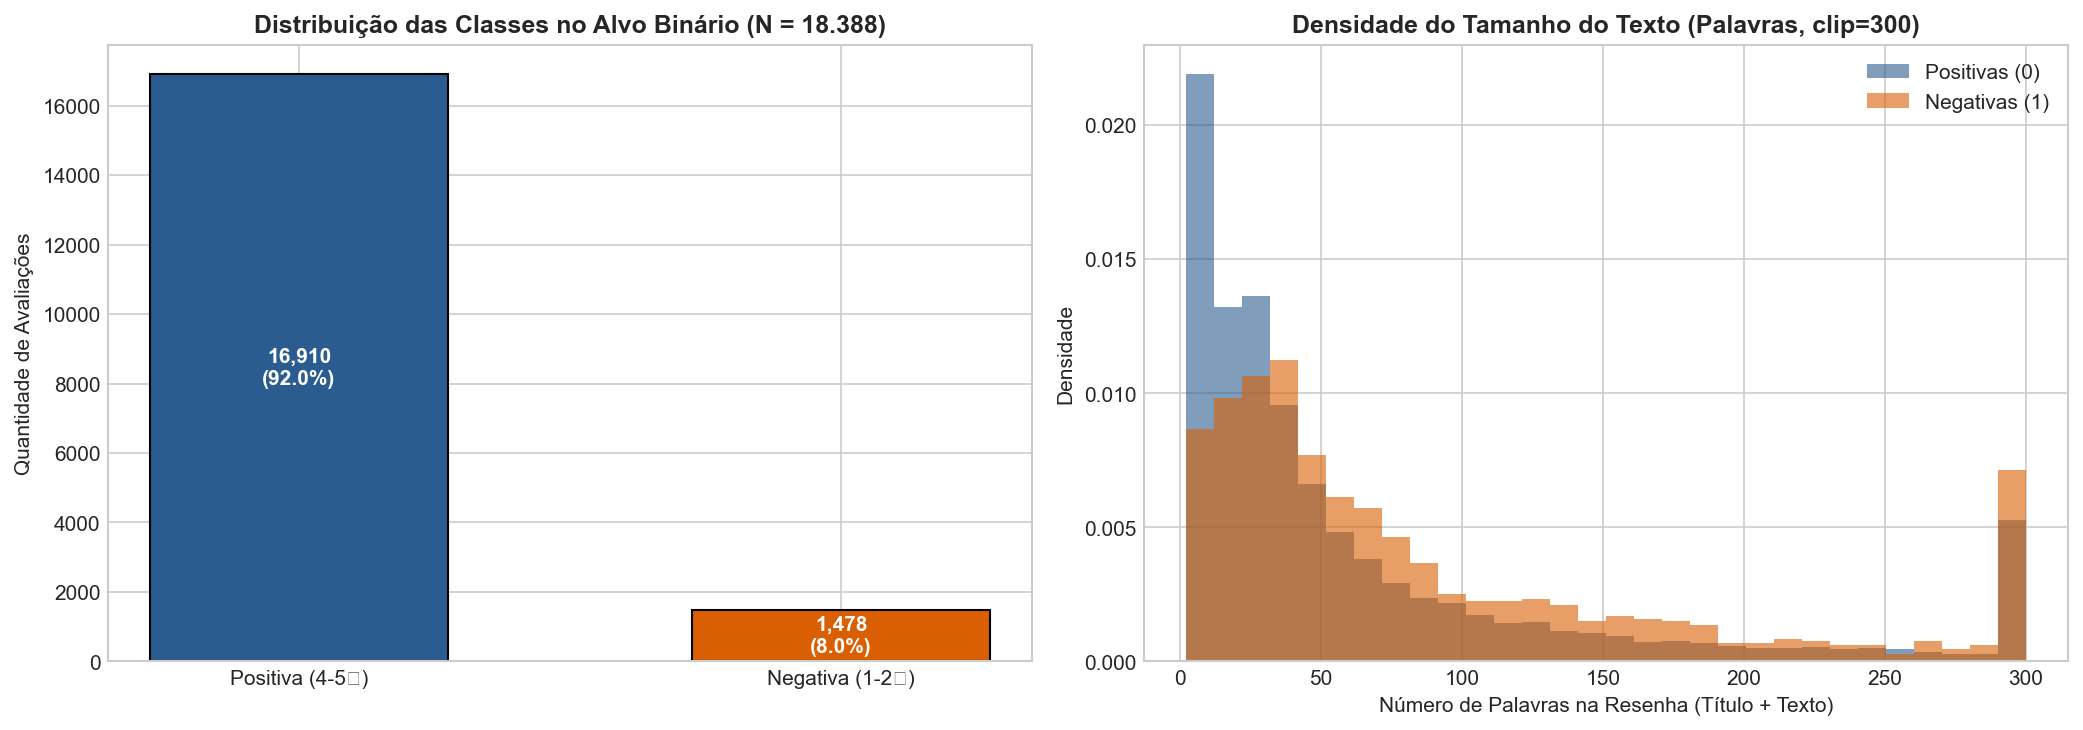
\includegraphics[width=\textwidth]{outputs/figura1_distribuicao_classes_eda.png}

{\tiny Distribuição de classes após binarização ($N=18.388$).}

\end{columns}

\vspace{0.18cm}

\begin{center}
\begin{beamercolorbox}[wd=0.96\textwidth, sep=0pt]{boxcinza}
  \begin{beamercolorbox}[wd=0.96\textwidth, ht=0.38cm, dp=0.08cm, leftskip=0.20cm]{boxtitulo}
    {\color{uelgreen}\scriptsize\textbf{Alerta Metodológico}}
  \end{beamercolorbox}
  \begin{beamercolorbox}[wd=\dimexpr0.96\textwidth-0.28cm\relax, sep=0.14cm]{boxcorpo}
    \scriptsize Acurácia simples é proibida: um classificador cego obteria \textbf{92\%} de acurácia sem detectar nenhuma insatisfação real.
  \end{beamercolorbox}
\end{beamercolorbox}
\end{center}

\end{frame}

% ==============================================================================
% Slide 4: Fluxo de Pensamento e Pipeline Anti-Vazamento
% ==============================================================================
\begin{frame}[t]{Fluxo de Pensamento e Pipeline Anti-Vazamento}

\textcolor{gray}{\small Prevenção estrita de \textit{Data Leakage} em todas as etapas}

\vspace{0.25cm}

\begin{center}
\begin{tikzpicture}[
    node distance=0.45cm,
    etapa/.style={rectangle, draw=uelgreen, thick, rounded corners, minimum width=1.65cm, minimum height=0.85cm, align=center, font=\tiny, fill=gray!8},
    seta/.style={->, thick, uelgreen}
]
\node[etapa] (s1) {1. Split 80/20\\Estratificado};
\node[etapa, right=of s1] (s2) {2. TF-IDF\\(\texttt{fit} no Treino)};
\node[etapa, right=of s2] (s3) {3. Seleção /\\Redução};
\node[etapa, right=of s3] (s4) {4. Classificador\\Balanceado};
\node[etapa, right=of s4] (s5) {5. Teste Cego\\($N=3.678$)};

\draw[seta] (s1) -- (s2);
\draw[seta] (s2) -- (s3);
\draw[seta] (s3) -- (s4);
\draw[seta] (s4) -- (s5);
\end{tikzpicture}
\end{center}

\vspace{0.25cm}

\scriptsize
\renewcommand{\arraystretch}{1.22}
\begin{center}
\begin{tabular}{P{2.7cm} P{6.8cm}}
\toprule
\textbf{Decisão} & \textbf{Justificativa Científica} \\
\midrule
Divisão prévia 80/20 & Treino ($14.710$) e Teste ($3.678$) separados antes de qualquer transformação (\texttt{random\_state=42}). \\
Tudo em \texttt{Pipeline} & Vocabulário, pesos $IDF$ e seletores ajustados estritamente dentro de cada fold da Validação Cruzada (5-fold). \\
Métrica orientadora & Foco em \textbf{F1-Score (Classe 1)}, \textbf{Recall} e \textbf{PR-AUC} devido ao desbalanceamento de $8{,}04\%$. \\
\bottomrule
\end{tabular}
\end{center}

\end{frame}

% ==============================================================================
% Slide 5: Mineração de Texto e Vetorização TF-IDF
% ==============================================================================
\begin{frame}[t]{Mineração de Texto e Representação TF-IDF}

\vspace{0.1cm}

\begin{itemize}
    \item \textbf{Engenharia de Texto:} \texttt{review\_full = title + " " + text}
    \begin{itemize}
        \item Títulos sintetizam a polaridade emocional da avaliação.
    \end{itemize}

    \vspace{0.2cm}

    \item \textbf{Parâmetros do \texttt{TfidfVectorizer} (dentro do Pipeline):}
    \begin{itemize}
        \item \textbf{Unigramas e Bigramas \texttt{(1, 2)}:} essenciais para capturar negações explícitas (\textit{``not good''}, \textit{``waste time''}).
        \item \textbf{Filtros de Frequência:} \texttt{min\_df=3} (remove erros raros de digitação) e \texttt{max\_df=0.90} (descarta termos onipresentes como \textit{``book''}).
        \item \textbf{Escala Sublinear (\texttt{sublinear\_tf=True}):} suaviza repetições em textos longos via $1 + \log(\text{TF})$.
        \item \textbf{Vocabulário:} limitado aos $5.000$ $n$-gramas mais relevantes.
    \end{itemize}
\end{itemize}

\vspace{0.2cm}

\begin{center}
\begin{beamercolorbox}[wd=0.96\textwidth, sep=0pt]{boxcinza}
  \begin{beamercolorbox}[wd=0.96\textwidth, ht=0.45cm, dp=0.08cm, leftskip=0.2cm]{boxtitulo}
    {\color{uelgreen}\scriptsize\textbf{Desafio da Alta Dimensionalidade Esparsa}}
  \end{beamercolorbox}
  \begin{beamercolorbox}[wd=0.96\textwidth, sep=0.2cm]{boxcorpo}
    \scriptsize Cada resenha ativa apenas uma fração mínima das $5.000$ dimensões. Métodos baseados em margem e regularização são decisivos nesse regime.
  \end{beamercolorbox}
\end{beamercolorbox}
\end{center}

\end{frame}

% ==============================================================================
% Slide 6: Modelagem Supervisionada (Linear SVM vs Regressão Logística)
% ==============================================================================
\begin{frame}[t]{Modelagem: Linear SVM vs. Regressão Logística}

\textcolor{gray}{\small Comparação em Validação Cruzada (5-Fold Estratificada no Treino)}

\vspace{0.2cm}

\begin{itemize}
    \scriptsize
    \item Ambos ajustados com \textbf{\texttt{class\_weight='balanced'}} para penalizar proporcionalmente os erros na classe minoritária (negativa).
\end{itemize}

\vspace{0.15cm}

\scriptsize
\renewcommand{\arraystretch}{1.25}
\begin{center}
\begin{tabular}{P{2.6cm} P{2.8cm} P{1.8cm} P{1.6cm}}
\toprule
\textbf{Modelo} & \textbf{Fundamentação} & \textbf{F1-Score (CV)} & \textbf{Desvio ($\sigma$)} \\
\midrule
\textbf{Linear SVM (\texttt{LinearSVC})} & Margem máxima (\textit{Hinge Loss}) & \textbf{0,6874} & $\pm 0{,}0189$ \\
\textbf{Regressão Logística} & Máxima verossimilhança (\textit{Log-Loss}) & 0,6851 & $\pm 0{,}0142$ \\
\bottomrule
\end{tabular}
\end{center}

\vspace{0.35cm}

\begin{center}
\begin{beamercolorbox}[wd=0.96\textwidth, sep=0pt]{boxcinza}
  \begin{beamercolorbox}[wd=0.96\textwidth, ht=0.45cm, dp=0.08cm, leftskip=0.2cm]{boxtitulo}
    {\color{uelgreen}\scriptsize\textbf{Escolha do Classificador Campeão}}
  \end{beamercolorbox}
  \begin{beamercolorbox}[wd=0.96\textwidth, sep=0.2cm]{boxcorpo}
    \scriptsize O \textbf{Linear SVM} ($C = 0{,}5$) foi selecionado por obter o maior F1-Score médio e por sua robustez matemática clássica para vetores TF-IDF esparsos de alta dimensão.
  \end{beamercolorbox}
\end{beamercolorbox}
\end{center}

\end{frame}

% ==============================================================================
% Slide 7: Seleção vs Redução de Atributos (Resultados)
% ==============================================================================
\begin{frame}[t]{Comparação: Seleção vs. Redução de Atributos}

\textcolor{gray}{\small Experimento controlado sobre o classificador campeão (Linear SVM, 5-Fold CV)}

\vspace{0.08cm}

\scriptsize
\renewcommand{\arraystretch}{1.12}
\begin{center}
\begin{tabular}{P{1.45cm} P{2.55cm} P{1.05cm} P{1.05cm} P{2.55cm}}
\toprule
\textbf{Versão} & \textbf{Técnica} & \textbf{F1 (CV)} & \textbf{Retenção} & \textbf{Diagnóstico} \\
\midrule
\textbf{Baseline} & Sem seleção ($5.000$ termos) & \textbf{0,6874} & \textbf{100\%} & Preserva cauda longa lexical \\
\textbf{Embedded} & \texttt{SelectFromModel} (L1) & 0,6614 & 96,2\% & Remove termos redundantes \\
\textbf{Filter} & \texttt{SelectKBest} ($\chi^2$, $1.500$) & 0,6472 & 94,2\% & Corta $70\%$ das variáveis \\
\textbf{Redução} & \texttt{TruncatedSVD} ($100$) & \textbf{0,4862} & 70,7\% & Queda severa ($\approx -30\%$) \\
\bottomrule
\end{tabular}
\end{center}

\vspace{0.04cm}

\begin{center}
\begin{beamercolorbox}[wd=0.96\textwidth, sep=0pt]{boxcinza}
  \begin{beamercolorbox}[wd=0.96\textwidth, ht=0.38cm, dp=0.06cm, leftskip=0.2cm]{boxtitulo}
    {\color{uelgreen}\scriptsize\textbf{Por que o SVD/PCA degradou o desempenho?}}
  \end{beamercolorbox}
  \begin{beamercolorbox}[wd=0.96\textwidth, sep=0.14cm]{boxcorpo}
    \scriptsize Em NLP esparso, palavras raras e pontuais (\textit{``waste''}, \textit{``horrible''}) carregam sinal preditivo direto. A projeção densa via SVD mistura essas palavras raras com termos comuns, diluindo o sinal no ruído ortogonal.
  \end{beamercolorbox}
\end{beamercolorbox}
\end{center}

\end{frame}

% ==============================================================================
% Slide 8: Visualização Seleção vs Redução
% ==============================================================================
\begin{frame}[t]{Impacto Visual: Seleção vs. Redução Dimensional}

\vspace{0.05cm}

\begin{center}
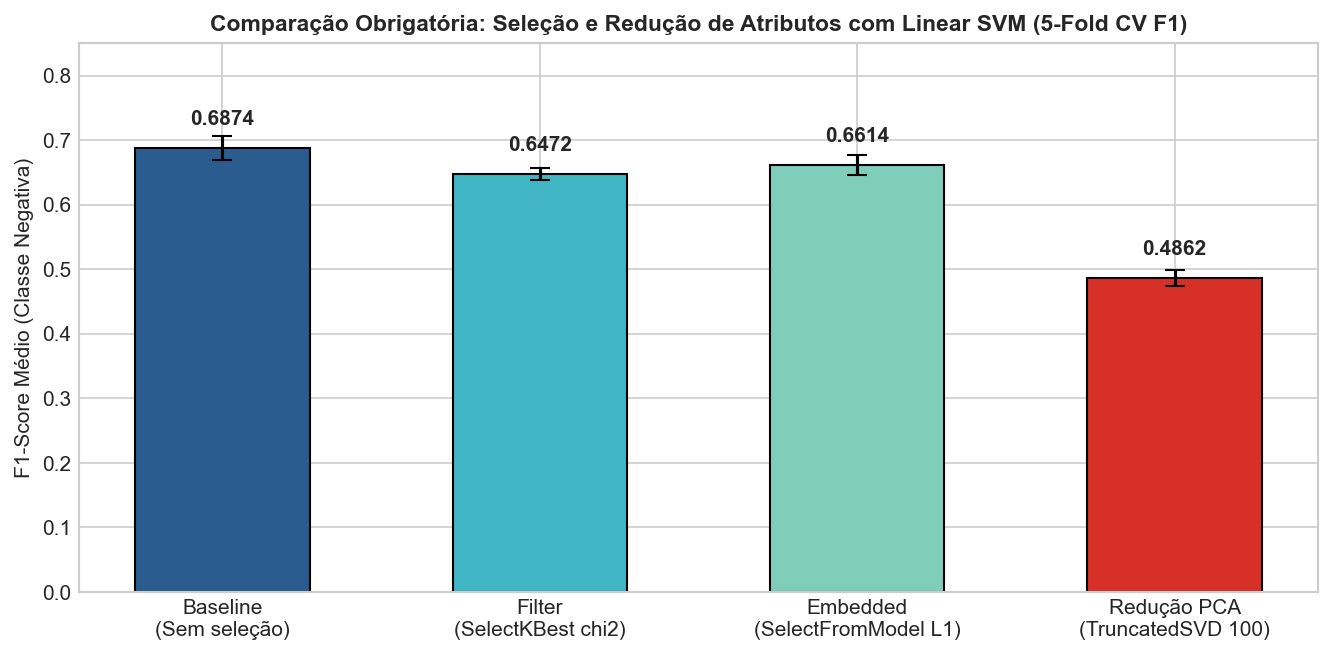
\includegraphics[width=0.76\textwidth]{outputs/figura3_comparacao_selecao_reducao.png}
\end{center}

\vspace{0.05cm}

\begin{center}
\scriptsize \textbf{Síntese:} Métodos de seleção (\textit{Filter} e \textit{Embedded}) mantêm $>94\%$ do desempenho original ao preservar termos discretos; a redução densa (\textit{TruncatedSVD}) destrói a separabilidade linear das críticas.
\end{center}

\end{frame}

% ==============================================================================
% Slide 9: Avaliação Final no Teste Cego
% ==============================================================================
\begin{frame}[t]{Avaliação Final no Conjunto de Teste Cego ($N = 3.678$)}

\textcolor{gray}{\small Execução única no conjunto de teste mantido intocado desde a etapa inicial}

\vspace{0.08cm}

\scriptsize
\renewcommand{\arraystretch}{1.12}
\begin{center}
\begin{tabular}{P{3.2cm} P{1.4cm} P{4.4cm}}
\toprule
\textbf{Métrica} & \textbf{Valor} & \textbf{Interpretação para o Negócio} \\
\midrule
\textbf{Recall (Classe Negativa)} & \textbf{77,70\%} & Detecta quase $8$ em cada $10$ insatisfações reais \\
\textbf{Precisão (Classe Negativa)} & \textbf{64,43\%} & $64\%$ dos alertas gerados são realmente negativos \\
\textbf{F1-Score (Classe Negativa)} & \textbf{0,7044} & Equilíbrio sólido sob severo desbalanceamento \\
\textbf{PR-AUC} & \textbf{0,7843} & Frente a $0{,}0805$ de baseline aleatório ($\approx 9{,}7\times$ maior) \\
\textbf{ROC-AUC} & \textbf{0,9689} & Alta separabilidade ordinal entre as classes \\
\bottomrule
\end{tabular}
\end{center}

\vspace{0.04cm}

\begin{center}
\begin{beamercolorbox}[wd=0.96\textwidth, sep=0pt]{boxcinza}
  \begin{beamercolorbox}[wd=0.96\textwidth, ht=0.38cm, dp=0.06cm, leftskip=0.2cm]{boxtitulo}
    {\color{uelgreen}\scriptsize\textbf{Balanço da Matriz de Confusão}}
  \end{beamercolorbox}
  \begin{beamercolorbox}[wd=0.96\textwidth, sep=0.14cm]{boxcorpo}
    \scriptsize Foram capturados \textbf{230 Verdadeiros Positivos (TP)} de insatisfação, contra apenas \textbf{66 Falsos Negativos (FN)} não detectados.
  \end{beamercolorbox}
\end{beamercolorbox}
\end{center}

\end{frame}

% ==============================================================================
% Slide 10: Gráficos de Avaliação no Teste
% ==============================================================================
\begin{frame}[t]{Matriz de Confusão e Curvas PR / ROC no Teste}

\vspace{0.05cm}

\begin{center}
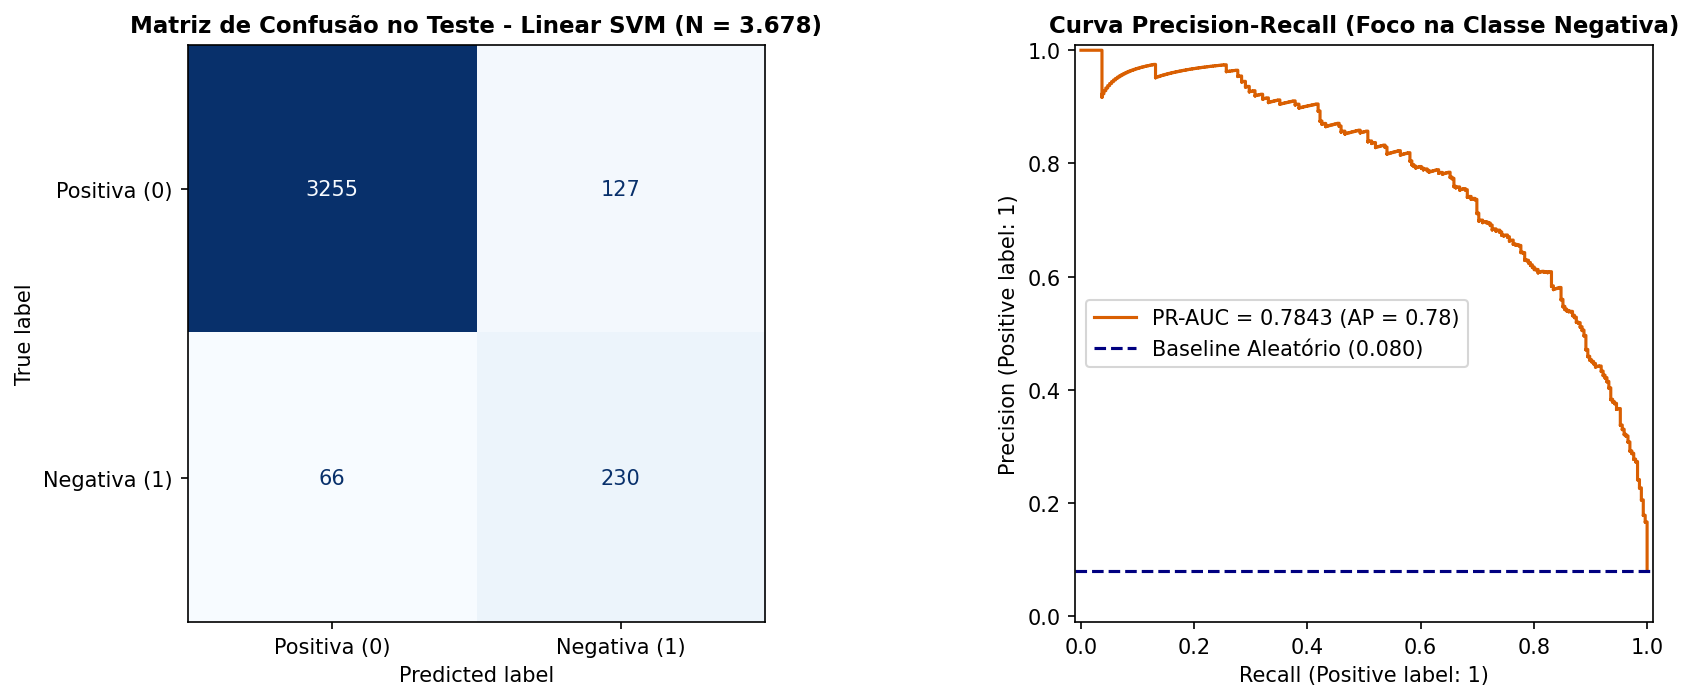
\includegraphics[width=0.92\textwidth]{outputs/figura4_avaliacao_matriz_confusao_pr_roc.png}
\end{center}

\vspace{0.05cm}

\begin{center}
\scriptsize O ganho expressivo em \textbf{PR-AUC (0,7843)} confirma que o modelo ordena com precisão as avaliações críticas no topo da fila de atendimento.
\end{center}

\end{frame}

% ==============================================================================
% Slide 11: Diagnóstico de Ruído e Estudo de Ablação (VADER)
% ==============================================================================
\begin{frame}[t]{Diagnóstico de Ruído nos Rótulos e Estudo de Ablação}

\begin{columns}[T]

\column{0.52\textwidth}
\begin{itemize}\setlength{\itemsep}{2pt}\setlength{\parskip}{0pt}
    \scriptsize
    \item \textbf{Diagnóstico VADER ($|\text{score}| \ge 0{,}60$):}
    \begin{itemize}\setlength{\itemsep}{1pt}
        \scriptsize
        \item Sinalizou \textbf{887 resenhas (4,82\%)} com contradição nota $\times$ texto (ex.: nota 1$\star$ com elogio).
        \item Tratadas como \textbf{suspeitas diagnósticas}, nunca como erros comprovados.
    \end{itemize}
    \vspace{0.08cm}
    \item \textbf{Ablação (remoção só no Treino):}
    \begin{itemize}\setlength{\itemsep}{1pt}
        \scriptsize
        \item Treino Normal ($14.710$): \textbf{F1 = 0,7044}
        \item Treino Filtrado ($13.999$): F1 = 0,6988
    \end{itemize}
\end{itemize}

\column{0.46\textwidth}
\centering
\vspace{0.1cm}
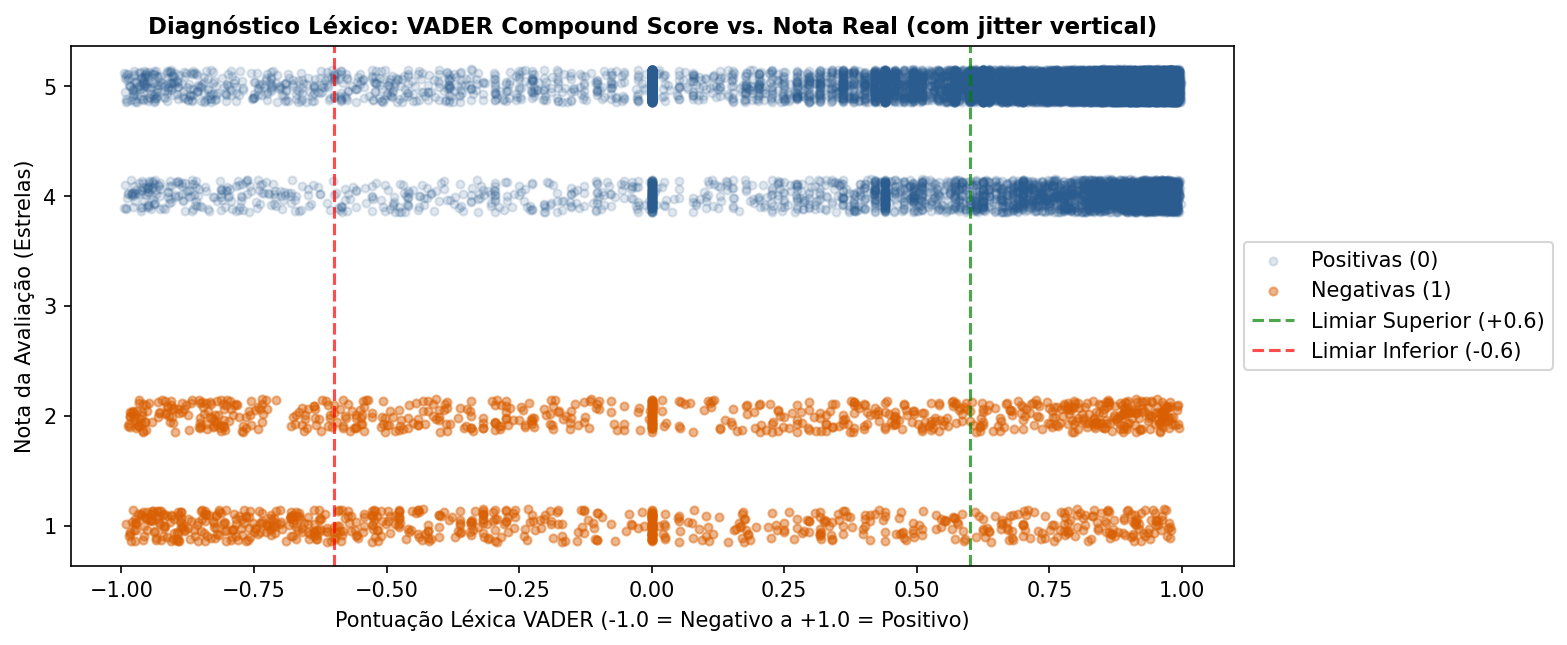
\includegraphics[width=\textwidth]{outputs/figura2_diagnostico_divergencias_vader.png}

{\tiny Divergências léxicas sinalizadas pelo VADER.}

\end{columns}

\vspace{0.18cm}

\begin{center}
\begin{beamercolorbox}[wd=0.96\textwidth, sep=0pt]{boxcinza}
  \begin{beamercolorbox}[wd=0.96\textwidth, ht=0.38cm, dp=0.08cm, leftskip=0.20cm]{boxtitulo}
    {\color{uelgreen}\scriptsize\textbf{Conclusão da Ablação}}
  \end{beamercolorbox}
  \begin{beamercolorbox}[wd=\dimexpr0.96\textwidth-0.28cm\relax, sep=0.14cm]{boxcorpo}
    \scriptsize O Linear SVM com TF-IDF já é naturalmente robusto ao ruído natural de rótulos; descartar amostras suspeitas piorou levemente o F1.
  \end{beamercolorbox}
\end{beamercolorbox}
\end{center}

\end{frame}

% ==============================================================================
% Slide 12: Interpretabilidade e Termos Mais Preditivos
% ==============================================================================
\begin{frame}[t]{Interpretabilidade: Termos Mais Preditivos}

\begin{columns}[T]

\column{0.56\textwidth}
\centering
\vspace{0.1cm}
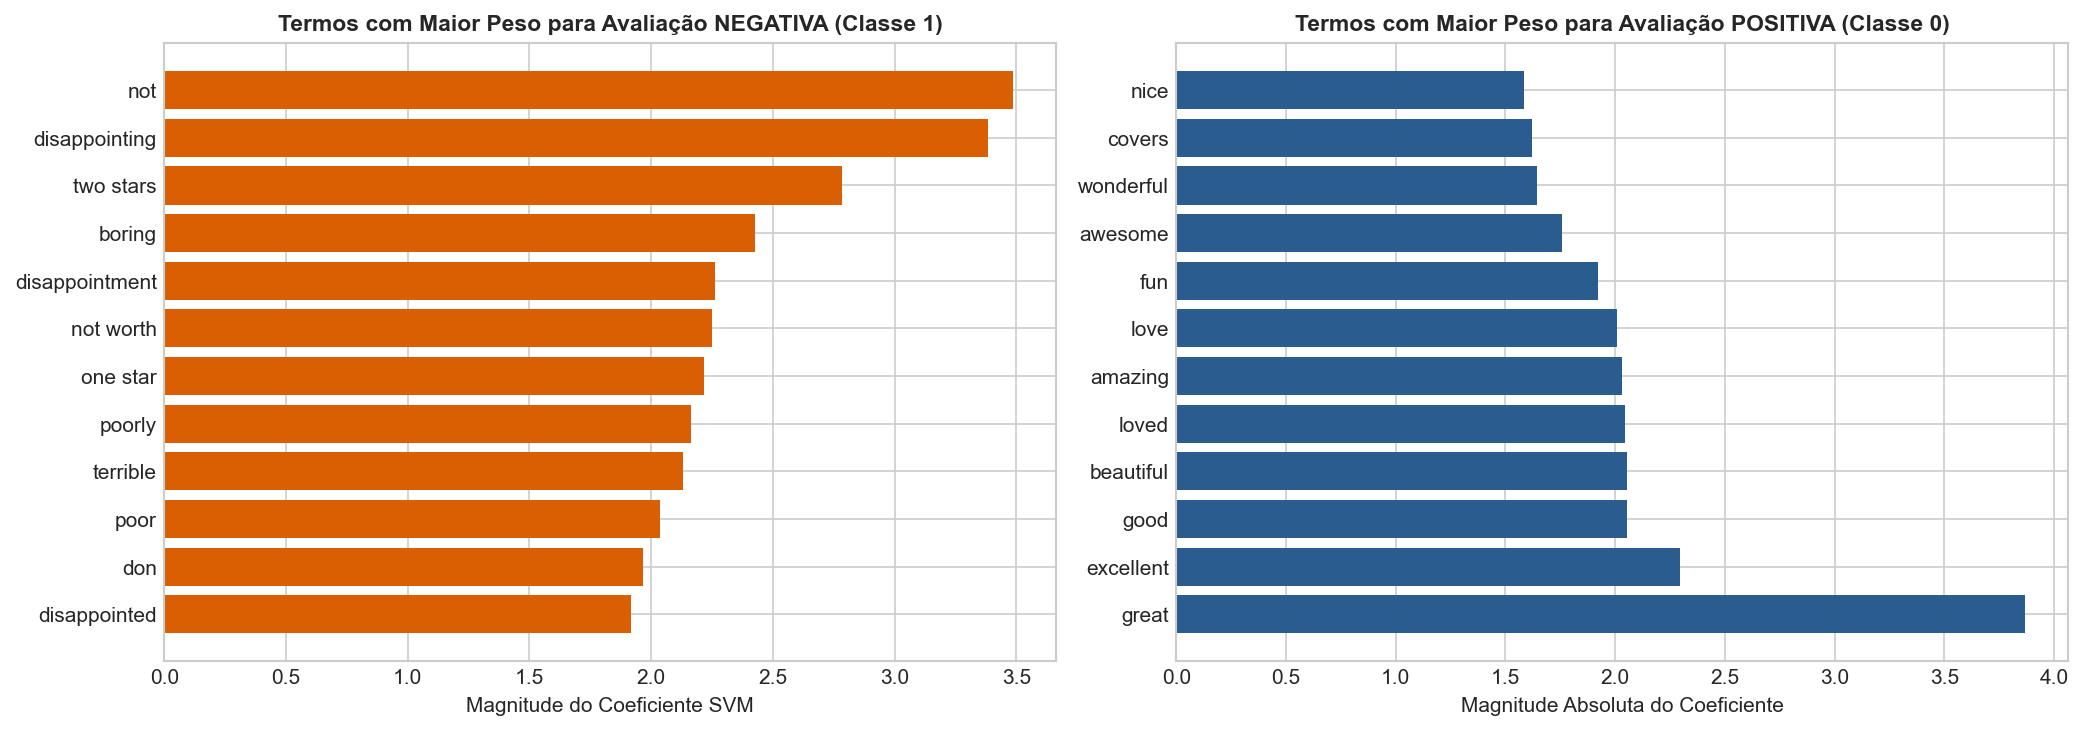
\includegraphics[width=\textwidth]{outputs/figura5_coeficientes_palavras_chave.png}

\column{0.42\textwidth}
\scriptsize
\textbf{Coeficientes do Hiperplano SVM:}
\begin{itemize}
    \item \textbf{Puxam para Negativa (Classe 1):} \\
    \textit{``waste''}, \textit{``not''}, \textit{``poor''}, \textit{``disappointed''}, \textit{``boring''}, \textit{``return''}, \textit{``waste time''}, \textit{``worst''}, \textit{``terrible''}, \textit{``awful''}.

    \vspace{0.15cm}

    \item \textbf{Puxam para Positiva (Classe 0):} \\
    \textit{``great''}, \textit{``excellent''}, \textit{``loved''}, \textit{``must read''}, \textit{``best''}, \textit{``highly recommend''}, \textit{``wonderful''}.
\end{itemize}

\vspace{0.15cm}

\begin{beamercolorbox}[wd=\textwidth, sep=0.15cm]{boxcinza}
    \scriptsize \color{uelgreen}\textbf{Destaque:} Bigramas como \textit{``waste time''} validam a inclusão de \texttt{ngram\_range=(1, 2)}.
\end{beamercolorbox}

\end{columns}

\end{frame}

% ==============================================================================
% Slide 13: Conclusão e Trabalhos Futuros
% ==============================================================================
\begin{frame}[t]{Conclusão Geral e Trabalhos Futuros}

\vspace{0.1cm}

\begin{center}
\begin{beamercolorbox}[wd=0.96\textwidth, sep=0pt]{boxcinza}
  \begin{beamercolorbox}[wd=0.96\textwidth, ht=0.45cm, dp=0.08cm, leftskip=0.2cm]{boxtitulo}
    {\color{uelgreen}\normalsize\textbf{Resposta à Pergunta de Pesquisa}}
  \end{beamercolorbox}
  \begin{beamercolorbox}[wd=0.96\textwidth, sep=0.22cm]{boxcorpo}
    \small \textbf{Sim.} É viável detectar avaliações negativas de livros com alta sensibilidade (\textbf{Recall de 77,7\%} e \textbf{PR-AUC de 0,784}) usando mineração de texto clássica e protocolo rigoroso sem vazamento de dados.
  \end{beamercolorbox}
\end{beamercolorbox}
\end{center}

\vspace{0.25cm}

\scriptsize
\begin{columns}[T]
\column{0.48\textwidth}
\textbf{Principais Entregas:}
\begin{itemize}
    \item Pipeline 100\% livre de \textit{data leakage}.
    \item Linear SVM superou Regressão Logística em base desbalanceada.
    \item Comprovação de que preservação lexical supera redução densa (SVD).
    \item Código e métricas reprodutíveis.
\end{itemize}

\column{0.48\textwidth}
\textbf{Trabalhos Futuros:}
\begin{itemize}
    \item Calibração de probabilidades (\texttt{CalibratedClassifierCV}).
    \item Ajuste fino do limiar de decisão conforme custo operacional do SAC.
    \item Avaliação com modelos neurais leves (ex.: \textit{DistilBERT}) como comparativo futuro.
\end{itemize}
\end{columns}

\end{frame}

% ==============================================================================
% Slide 14: Referências
% ==============================================================================
\begin{frame}[t]{Referências}

\vspace{0.3cm}

\scriptsize
\begin{beamercolorbox}[wd=0.96\textwidth, sep=0.25cm]{boxcorpo}

HOU, Y. et al. \textbf{Bridging Language and Items for Retrieval and Recommendation (Amazon Reviews 2023)}. McAuley Lab / UCSD, 2024. Disponível em: \url{https://amazon-reviews-2023.github.io/}.

\vspace{0.22cm}

JOACHIMS, T. \textbf{Text Categorization with Support Vector Machines: Learning with Many Relevant Features}. In: ECML, 1998.

\vspace{0.22cm}

HUTTO, C. J.; GILBERT, E. \textbf{VADER: A Parsimonious Rule-Based Model for Sentiment Analysis of Social Media Text}. In: ICWSM, 2014.

\vspace{0.22cm}

PEDREGOSA, F. et al. \textbf{Scikit-learn: Machine Learning in Python}. Journal of Machine Learning Research, v. 12, p. 2825--2830, 2011.

\vspace{0.22cm}

REPOSITÓRIO DO PROJETO. \textbf{Mineração de Dados (2COP024) --- UEL}. Disponível em: \url{https://github.com/luticaa/mineracao-de-dados-projeto-final}.

\end{beamercolorbox}

\end{frame}

\end{document}
